\section{Implicit Solvent Models}\label{sec:implicit}
\vspace{3cm}
\par
As it is mentioned in Section \ref{sec:MD}, interactions between a solute molecule and a surrounding solvent are of fundamental importance across chemistry, biology, and associated fields of science and engineering. Fully atomistic, explicit-solvent MD simulations provide an accurate and chemically detailed understanding of these interactions therefore they can be can be highly demanding in the consumption of computational resources. This cost is is associated with the large number of solvent molecules required to model a bulk solution. In practical situations, a large fraction of the time is spent calculating a detailed trajectory of the solvent molecules, even though it is primarily the solute behavior that is of interest.

Because of this, it is desirable to develop different approaches in which the influence of the solvent is incorporated \textbf{implicitly}. Approximate schemes treating the solvent implicitly can provide useful quantitative estimates and remain computationally inexpensive \cite{roux1999implicit} \cite{zacharias2003continuum}.

\subsection{Implicit model: Solvation Free Energy}

Solvation is the process of reorganizing solvent and solute molecules into solvation systems. Solvation involves bond formation, hydrogen bonding, and van der Waals forces. Solvation of a solute by water is called hydration \cite{campbell2006chemistry}. The solvation process describes the interaction between the solute and solvent molecules. This process will be thermodynamically favored only if the overall Gibbs energy of the solution is decreased, compared to the Gibbs energy of the separated solvent and solid (or gas or liquid). Regarding Equation \ref{eq:Gibbs}, a negative Gibbs energy indicates a spontaneous process but does not provide information about the rate of dissolution.

This process involves multiple steps with different energy consequences: First, a cavity must form in the solvent to make space for a solute (Figure \ref{fig:solv_1} to Figure \ref{fig:solv_2}). This is both entropically and enthalpically unfavorable, as solvent ordering increases and solvent-solvent interactions decrease. Stronger interactions among solvent molecules leads to a greater enthalpic penalty for cavity formation. Next, a particle of solute must separate from the bulk. This is enthalpically unfavorable since solute-solute interactions decrease, but when the solute particle enters the cavity, the resulting solvent-solute interactions are enthalpically favorable. 

\begin{figure}[h]
    \centering
    \begin{subfigure}[t]{0.25\textwidth}
    
\includegraphics[width=\textwidth]{Figures/Chapter 4/Cavity_1.png}
    \caption{Representation of bulk solvent.}
    \label{fig:solv_1}
    \end{subfigure}
    \hspace{0.5cm}
    \begin{subfigure}[t]{0.25\textwidth}
    
\includegraphics[width=\textwidth]{Figures/Chapter 4/Cavity_2.png}
    \caption{A cavity with the solute geometry is form in the solvent.}
    \label{fig:solv_2}
    \end{subfigure}
    \hspace{0.5cm}
    \begin{subfigure}[t]{0.25\textwidth}
    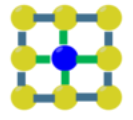
\includegraphics[width=\textwidth]{Figures/Chapter 4/Cavity_3.png}
    \caption{The solute is placed in the solvent cavity with the respective solute-solvent interactions}
    \label{fig:solv_3}
    \end{subfigure}
   
    \caption{Representation of the solvation process for any molecule in solution.}
    \label{fig:solvation}
\end{figure}
The solvation free energy, process described in Figure \ref{fig:solvation}, is frequently decomposed as a sum of \textit{polar} $(\Delta G_{polar})$ and \textit{non-polar} $(\Delta G_{np})$ terms  \cite{zacharias2003continuum}. 
\begin{equation}
    \Delta G^{solv} = \Delta G_{polar}^{solv} + \Delta G_{np}^{solv}
    \label{eq:G_solv}
\end{equation}
The polar term is the free energy of creating the solute’s charge distribution inside a pre-existing solute cavity, Assuming a charge distribution given by a molecular mechanics force field, the polar solvation contribution can be modeled with macroscopic continuum dielectric theory, e.g. the Poisson-Boltzmann equation. This works focuses on the \textbf{non-polar} component which is define as the work required to place an uncharged solute inside the solvent and generates a dry cavity on it. This contribution is often estimated from the solvent accessible surface area (SASA) of the molecule using a uniform surface tension coefficient obtained from a fit of experimental \cite{zacharias2003continuum}. 

\subsubsection{Solvent-Accessible Surface Area (SASA) Model}\label{subsubsec:SASA_model}
Implicit-solvent models often treat $\Delta G_{np}$ as a weighted combination of the solute’s SASA and other geometric measures given by: 
\begin{equation}
    \Delta G_{np} = \gamma (SASA) + b
    \label{eq:SASA}
\end{equation}
where $\gamma$ is is usually interpreted as the liquid-vapor surface tension, and $b$ is a scaling constant. Geometrically, \textit{Solvent Accessible Surface Area} is related to the region of the molecule surface exposed enough to be able to interact with solvent molecules. It is usually defined as a surface built by the delineation drawn by the center of a sphere (rough representation of a solvent molecule, usually of 1.4 [\r{A}] radii; i.e. a water molecule) rolling over the molecular surface. 
Nevertheless, the accurate prediction of the solvation free energy remains a very challenging issue and several inaccuracies with this method have been presented by some authors \cite{gallicchio2000enthalpy} \cite{wang2018breaking},  suggesting that an empirical parametrization of the hydration free energy and the free energy of association of apolar species based only on the solvent accessible surface area is insufficient. Successful parametrization should contain a surface area term to reproduce effects due to entropy loss and solvent reorganization energy and terms that depend on the number, location, and type of atomic interaction centers to reproduce effects due to the solute-solvent dispersion interactions which are only weakly correlated with surface area. 










\subsection{Non-polar Solvation Free Energy Estimation}\label{subsec:CC_method}

The non-polar term in Equation \ref{eq:G_solv} can itself be decomposed into a sum of two free energies \cite{zacharias2003continuum}, $\Delta G_{cav}$ the creation of a solute-shaped cavity by turning on the potential short-range \textbf{repulsive interactions}, and $\Delta G_{disp}$, in which one turns on the longer-range \textbf{attractive} solute-solvent dispersion interactions.
\begin{equation}
    \Delta G_{np}=\Delta G_{cav} + \Delta G_{disp}
    \label{eq:G_np}
\end{equation}
Traditionally, $\Delta G_{cav}$ is highly correlated with the SASA factor previously described, however, the value of $\gamma$ does not agree with the surface tension coefficient and works as a adjustable parameter which can change the errors. On the other hand, $\Delta G_{disp}$ can be described with a continuum model, where the solute-solvent dispersion interaction potential is integrated over the solvent, which in turn can be formulated as an volume integral over the solvent accessible surface \cite{tan2007implicit}.
It is been study that while repulsive and attractive components of the non-polar part both scale roughly with surface area (or volume) of the solute, the total non-polar free energy does not scale with the solute surface area or volume. \cite{mobley2009small}.

\subsubsection{Implicit Solvent Model for $\Delta G_{cav}$ and $\Delta G_{disp}$}
A new approach to estimate $\Delta G_{cav}$ and $\Delta G_{disp}$ \cite{} proposes an implicit solvent model with a clearer physical meaning than current available models. Regarding Equations \ref{eq:G_solv} and \ref{eq:G_np}, the non-polar solvation free energy can be expressed as (See Figure \ref{fig:np_cycle}): 
\begin{equation}
    \Delta G_{solv}= \Delta G_{cav}+ \Delta G_{disp}+ \Delta G_{polar}
\end{equation}
\begin{figure}[h]
    \centering
    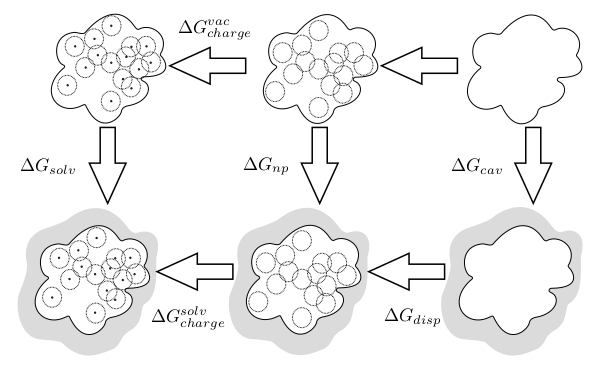
\includegraphics[scale=0.6]{Figures/Chapter 4/np_cycle.png}
    \caption{Thermodynamic cycle for solvation energy. Figure taken from \cite{cooper2020simple}}
    \label{fig:np_cycle}
\end{figure}

Using a capacitance-based approach for $\Delta G_{cav}$, the potential inside the solute is model as a constant $\phi_{static}$, defining the solute boundary as the solvent-excluded surface (SES) \cite{connolly1983analytical}. In the infinite solvent region, the potential is model as $\phi=0$, and bound the region using the boundary of the first solvation shell (the solvent-accessible surface, SAS \cite{connolly1983analytical}. These surfaces bound a shell, which is model as a macroscopic dielectric with the uniform relative permittivity $\epsilon_{shell}$, and where the electrostatic potential obeys the Laplace equation. Fixing the potentials at both boundaries implies that the dielectric constants of the solute and bulk solvent are irrelevant.. It is used $\epsilon_{shell}$ as a fitting parameter, but it has clear physical bounds and significance. The energy associated with this boundary-value problem can be solved using a pair of coupled boundary-integral equations for unknown charge densities on the two surfaces by: 
\begin{equation}
    \begin{bmatrix}
V_{diel} & V_{diel}\\ 
 V_{shell}& V_{shell}
\end{bmatrix}\begin{bmatrix}
\sigma_{diel}\\ 
\sigma_{shell}
\end{bmatrix}
=
\begin{bmatrix}
\phi_{static}\\ 
0
\end{bmatrix}
\end{equation}
where $V_{diel}(\phi_{shell})=\oint_{shell}\frac{\phi(r')}{4\pi\left |r_{diel}-r' \right |}$ denotes the potential induced at the inner surface (the dielectric boundary) by the surface charge distribution on the outer boundary (the solvent-accessible surface). Figure \ref{fig:capacitor} represent this idea. 
\begin{figure}[h]
    \centering
    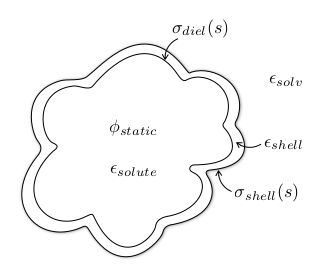
\includegraphics[scale=0.5]{Figures/Chapter 4/capacitor_model.png}
    \caption{Sketch of the capacitor model. Figure taken from \cite{cooper2020simple}}
    \label{fig:capacitor}
\end{figure}
Having found the surface charge distributions it is possible to compute the work (and hence, the free energy) required to charge the resulting capacitor with standard electrostatic theory
\begin{equation}
    \Delta G_{cav}=\int_{\Omega}\phi(r)\rho(r)dr
    \label{eq:g_cav}
\end{equation}
being $\rho$ the charge distribution, in this case, concentrated on the SAS ($\sigma_{shell}$) and SES ($\sigma_{diel}$)Noting that the potential on the outer surface is zero, we can rewrite Equation \ref{eq:g_cav} as: 
\begin{equation}
    \Delta G_{cav}=\oint_{diel}\phi_{static}\sigma_{diel}(r)dr
    \label{eq:int_shell}
\end{equation}

The previous $\Delta G_{cav}$ component is combine with a modification of a continuum integral method \cite{levy2003nonpolar} for calculating $\Delta G_{disp}$, by integrating the Lennard-Jones potential outside the solvent-accessible surface which can be formulated as a surface integral using the divergence theorem by: 
\begin{equation}
    \Delta G_{disp}=\sum_i \oint_{shell} \rho_w \frac{\partial}{\partial n}\left ( \frac{A_i}{90\left |r-r_i\right |^{10}} - \frac{B_i}{12\left |r-r_i\right |^{4}} \right )dr
    \label{eq:CC_implicit}
\end{equation}
where $\rho_w$ is considered to be the bulk number density, $A_i$ and $B_i$ re related to the Lennard-Jones parameters for the water oxygen and atom i, the sum is over the solute’s atoms, and the unit vector \textbf{n} points into the solvent.
Finally, a solvation-layer interface condition (SLIC) continuum electrostatics method   \cite{mehdizadeh2019solvation} is used to compute $\Delta G_{polar}$ (or $\Delta G_{charge}^{solv}$ in Figure \ref{fig:np_cycle}). (Notice that regarding the thermodynamic cycle represented in Figure \ref{fig:np_cycle},  $ \Delta G_{solv}$ is equivalent to $\Delta G_{charge}^{solv}$ - $\Delta G_{charge}^{vac}$).



 